\chapter{Introduction} \label{ch:introduction}
\section{Statistical Physics}
Statistical physics is a field of study with its roots in thermodynamics. The initial goal was to understand the thermal properties of matter and the behavior of gases \cite{Kardar}. It has been studied since the 1600's with contributions coming from such prominent physicists as Bernoulli, Maxwell, and Boltzmann \cite{Flamm1998}. Initial studies of the topic  revolved around the understanding of heat processes and engines. These are systems that contain moles of particles interacting with their environment, like heat reservoirs. As technology increased, scientists began to test these statistical theories at lower and lower temperatures. Eventually, the discovery of phenomena such as superconductivity and superfluidity led to the necessity of a new theoretical picture in order to describe the underlying physics. The theory of quantum mechanics explains these phenomena with the help of statistical mechanics. Experimentalists are now at the point where temperatures as low as micro Kelvin are used in experiments \cite{Onofrio2016, Es2010,Bhar}. This technology has given rise to the study of atoms in cold and ultra cold environments. These experiments are perfect testing grounds for some of the fundamental quantum mechanical problems that show up in undergraduate and graduate textbooks. 

\section{Quantum Mechanical Traps} \label{section:QMtraps}
In cold atom experiments, cold atomic clouds are placed into a region containing a potential \cite{Bhar}. To understand how these clouds behave, it's necessary to look at some of the potentials that are applied in these experiments. Two example potentials are the harmonic oscillator and the infinite potential well. The energy eigenvalues can be found by solving the Schr\"odinger which is shown in Appendix \ref{section:appendixA}. These eigenvalues give the linear spectrum 
\begin{equation}
    E_i=\hbar\omega\qty(i+\frac{1}{2}) \label{SHOpot}
\end{equation}
for the simple harmonic oscillator and quadratic equation 
\begin{equation}
    E_i=\frac{(i+1)^2\pi^2\hbar^2}{2ma^2} \label{quadpot}
\end{equation}
for the infinite potential well, where $a$ is the length of the well and $i=0,1,2,3,...$. The term $i$ is a positive integer that identifies allowed energy levels to solve the Schr\"odinger equation for the two potentials mentioned.

Since these gases are composed of a single atomic species, either bosons or fermions, they are identical. 
The density of the gas is typically around $10^5 \text{cm}^{-3}$ \cite{Viering} but can get as high as $10^{12} \text{cm}^{-3}$ \cite{Radwell}. 
Being neutral atoms, the only interaction to worry about is the Van der Waals force. 
This force is typically present at length scales of Angstroms ($10^{-10}$m) \cite{biochem}. 
Specifically for Potassium and Rubidium, the length scale is $3.13\rm \AA$ \cite{Pot} and $4.48\rm \AA$ \cite{Rub} respectively. 
Using the two values above as the range, the mean interparticle distance is between $\qty(\frac{1}{10^5})^{1/3}\approx 2.15$mm and $\qty(\frac{1}{10^{12}})^{1/3}\approx 10 \mu$m. With these values, the Lennard-Jones potential can be found for each. For Potassium, this value is $U\approx-5.298\times 10^{-43}$eV for an interparticle distance of $2.15$mm and $U\approx-5.233\times 10^{-29}$eV for an interparticle distance of $10 \mu$m. Likewise for Rubidium, $U\approx-1.1088\times 10^{-41}$eV for an interparticle distance of $2.15$mm and $U\approx-1.095\times 10^{-27}$eV for an interparticle distance of $10 \mu$m. In Viering's Rubidium experiment, a linear spectrum was created with a gap size of $\hbar\omega\approx 4.136\times 10^{-12}$eV \cite{Viering}. This gap size is much larger than the possible values of the Lennard-Jones potential for Rubidium. 

This shows that even if two particles were to interact via van der Waals, there is not enough force to change the energy state of either interacting particle. For this reason, it is acceptable to consider these gases as non-interacting. 
The non-interaction restriction is essential because it allows for the use of the single particle spectra that are considered in Eqs.\@ (\ref{SHOpot}) and (\ref{quadpot}). 
If interactions are considered, the Hamiltonians used to derive Eqs.\@ (\ref{SHOpot}) and (\ref{quadpot}) will change. 
This will require the new Hamiltonians to be rediagonalized. 
This is not something realistic to calculate for these cold atom systems because their Hilbert space is infinite. 
In many experiments, the simple harmonic oscillator potential can be realized with a magneto-optical trap \cite{Bhar, Viering, Radwell,Phillips_1998}. 
The development of this method won the Nobel prize in 1997 for its impact on the physics community \cite{nobelprize.org_1997}. 
More recently, the potential well has been realized by transferring atoms onto an atomic chip \cite{Es2010}. 
There are other traps that consist of more exotic shapes, like a trap that is a box in two dimensions (say the x-z and x-y planes) and circular in the other (say the x-y plane) \cite{Mukherjee2017}. 
After these atoms are placed into the trap, they can be probed using the time of flight (TOF) method. To summarize this method, the atoms are released from the trap by turning it off, and the velocity distribution of the trapped atoms is measured \cite{Brzozowski,Wheeler_2003}. This probability distribution of velocities is utilized to extract the single particle occupation numbers, i.e. the number of particles in each energy state $i$ as described above. Then to find the temperature of these distributions, experimentalists use statistical mechanics to fit the data to a prediction from a statistical ensemble. This procedure is essential to extracting the temperature at these ultra-low densities since conventional thermometry, which requires interactions, is not possible. 


\section{Ensemble Theory for Non-interacting Identical Particles}
The thermodynamic properties of a cold atomic cloud can be derived using statistical mechanics. For a large system of particles, this introduces many degrees of freedom, so the states of the system are described in the context of ensembles. 
An ensemble is a grouping of microstates that corresponds to a mixed macrostate \cite{Kardar}. A microstate is a particular configuration of particles in the system. For example, if a box has two coins in it, shaking the box can only produce four states, $(H,H),(H,T),(T,H),(T,T)$ \cite{Blundell}. These are the microstates of the system.
A macrostate is the collection of all microstates that give a specific equilibrium condition. Going back to the coin example, there are three macrostates, both heads, both tails, and a head and a tail. The last macrostate consists of the two microstates $(H,T)$ and $(T,H)$ since they each contain a head and a tail. These macrostates can then be analyzed as an ensemble. 

There are three ensembles that are used in statistical mechanics, the microcanonical, canonical, and grand canonical ensembles. The microcanonical ensemble describes a system that is mechanically and adiabatically isolated \cite{Kardar}. This means the system is disconnected from any sort of heat or work that could be applied or extracted. Since there's no input or output, the internal energy is fixed and as a result, the equilibrium temperature is also fixed. 
The canonical ensemble describes a system that allows heat and work to be an input. This ensemble is usually modelled as a system that is in contact with a reservoir that's large enough  that interactions between the two do not affect the reservoir's temperature. 
The grand canonical ensemble is similar to the canonical ensemble except now it allows chemical work to be done. In the language of thermodynamics, the chemical potential $\mu$ is defined as 
\begin{equation*}
    \mu=\qty(\frac{\partial U}{\partial N})_{S,V}
\end{equation*}
where $U$ is the internal energy, $N$ is the particle number, $S$ is the entropy, and $V$ is the volume. The subscript $S$ and $V$ state that the entropy and the volume of the system are held constant \cite{Blundell}. This gives the chemical potential as the change in energy with respect to the number of particles present. The chemical potential is needed because it allows for the change in number of particles in the system. 

An example of this would be trying to describe heating a classroom. In this case, the number of particles is allowed to vary, like particles leaving and entering through the door of the classroom. In this scenario, it is appropriate to find the equilibrium temperature by using the grand canonical ensemble to account for the change in particle number. Since the exact number of particles changes at any point in time, it makes more sense instead to describe the average number of particles $\avg{N}$. 

When working with the canonical and grand canonical ensemble, it is also necessary to 
define a normalization factor for the Boltzmann probabilities that show up. This normalization factor is called the partition function, which is a function of thermodynamic state variables that is defined as a sum over all the states of Boltzmann factors \cite{Blundell}. In other words, it is a Boltzmann distribution that is related to thermodynamic variables such as temperature. This function is used to derive thermodynamical properties of the system, like specific heat and internal energy. 
To calculate the partition function, an ideal quantum gas of non-interacting identical particles will be considered. This will allow for a theoretical analysis of the cold atom clouds that were considered in the previous section. With this motivation, we begin with an analysis of the canonical ensemble. The partition function in the canonical ensemble is written as
\begin{equation}
    Z_N=\sum_{\{n_i\}}^{'} \exp\qty[-\beta\sum_{i} \epsilon_i n_i]=\sum_{\{n_i\}}^{'} \prod_i \exp\qty[-\beta\epsilon_i n_i]
\end{equation}

\begin{equation}  
    \sum_i n_i=N.
\end{equation}

\textbf{In this project, we will only consider systems of ultracold fermions where the number of particles that can occupy a given single-particle state is restricted to $\bold{n_i=\{0,1\}}$ due to the Pauli exclusion principle. This fermionic constraint will be assumed in all expressions.} 
This constraint makes the summation very difficult to calculate since there are many ways to select microstates (occupation states of particles) to get an specific value of $N$. To remove this restriction, the grand canonical ensemble can be employed. The grand canonical partition function is written as 
\begin{align}
    Z_{GC}&\equiv\sum_{N=0}^{\infty} \exp(\beta\mu N) \sum_{\{n_i\}}^{'} \prod_i \exp\qty[-\beta\epsilon_i n_i]\nonumber\\
    &=\sum_{N=0}^{\infty}\sum_{\{n_i\}}^{'} \exp(\beta\mu N) \prod_i \exp\qty[-\beta\epsilon_i n_i]\nonumber\\
    &=\sum_{\{n_i\}} \prod_i \exp(\beta\mu n_i) \exp\qty[-\beta\epsilon_i n_i]\nonumber\\
    &=\sum_{\{n_i\}} \prod_i \exp\qty[-\beta\qty(\epsilon_i-\mu)n_i]
\end{align}
where the removal of the prime in the summation over $\{n_i\}$ indicates that there is no restriction on the value of $N$ after the application of the infinite sum over the number of particles. The first line of the steps above can be rewritten to relate the canonical ensemble to the grand canonical ensemble as
\begin{equation}
    Z_{GC}=\sum_{N=0}^{\infty} e^{\beta\mu N} Z_N.
\end{equation}
 The important step here is the inclusion of the chemical potential. The summation over the chemical potential term considers $N$ particles ranging from zero to infinity. This fixes the problem with the restricted summation in the canonical ensemble, which is going over all possible configurations to get $N$ particles. With the inclusion of the infinite sum, $N$ can take any value, so the primed summation becomes unrestricted. The two exponential terms can be simplified and the grand canonical partition function is written as 
\begin{equation}
    Z_{GC}=\sum_{\{n_i\}} \prod_i \exp\qty[-\beta\qty(\epsilon_i-\mu)n_i] \label{ZGC}
\end{equation}
and for fermions, we can explicitly perform the sum over the two possible occupations $n_i=\{0,1\}$ to yield:
\begin{equation}
    Z_{GC}=\prod_{i}\qty[1+\exp(-\beta\qty(\epsilon_i-\mu))]. \label{ZGCferm}
\end{equation}
To make connection with experimental time of flight measurements of the single particle occupation numbers, we consider the mean number of particles in the grand canonical ensemble. Using Eq.\@ (\ref{ZGC}), this is 
\begin{align}
    \avg{n_i}_{GC}&=\frac{\sum_{\{n_j\}} n_i \prod_j \exp(-\beta n_j(\epsilon_j-\mu))}{Z_{GC}}\nonumber\\
    &=\frac{-1}{Z_{GC}}\frac{\partial Z_{GC}}{\partial (\beta\epsilon_i)}\nonumber\\
    &=-\frac{\partial \ln(Z_{GC})}{\partial (\beta \epsilon_i)}. \label{avgnum}
\end{align}
Using Eq.\@ (\ref{avgnum}), this can be solved to find 
\begin{align}
    \avg{n_i}_{GC}&=-\frac{\partial}{\partial (\beta\epsilon_i)} \sum_i \qty[1+\exp(-\beta\qty(\epsilon_i-\mu))]\nonumber\\
    &=\frac{\exp(\beta(\mu-\epsilon_i))}{1+\exp(\beta(\mu-\epsilon_i))}\nonumber\\
    &=\frac{1}{1+\exp(-\beta(\mu-\epsilon_i))}. \label{GCoccprob}
\end{align}
This equation can be used to define the complement as
\begin{equation}
    \avg{\Bar{n}_i}=1-\avg{n_i}_{GC}=\frac{1}{1+\exp(-\beta(\epsilon_i-\mu))}. \label{GCcomplement}
\end{equation}
We recognize this to be the same term inside the product of Eq.\@ (\ref{ZGCferm}) which allows it to be written as 
\begin{equation}
    Z_{GC}=\prod_i \frac{1}{\avg{\Bar{n}_i}}. \label{GCq}
\end{equation}

The benefit of using the grand canonical ensemble is shown in this equation. 
For non-interacting fermions, the grand canonical partition function can be found from a simple product that has no restrictions with the average number of particles being enforced by the chemical potential, while the canonical ensemble requires that the particle number condition be met. 
As previously mentioned, the probability distributions are calculated from the velocity distribution measured from the TOF in cold atom experiments. To extract temperature from the probability distribution, it is easy to fit the data to Eq.\@ (\ref{GCcomplement}) and extract $\beta$ and a formally unphysical value of $\mu$. Further, the data can be used to find the grand canonical partition function which can be used to find other thermodynamic properties of the system, like internal energy or specific heat. In the thermodynamic limit, that is when the number of particles is large. The two ensembles are equivalent so there is no error in fitting the data to the grand canonical ensemble. 
However, in the latest generation of cold atom experiments that are considered in Section \ref{section:QMtraps}, the conditions for the thermodynamic limit are not met as the number of particles in the system could be on the order of $10^{4}-10^{5}$ and has a fixed value. Therefore, the correct ensemble to use is the canonical as it describes a system with a fixed number of particles. To understand the error in the common use of the grand canonical ensemble to describe a canonical system, we begin by considering a simple example. 


\section{Simple Example}\label{section:simpleexample}
Away from the thermodynamic limit, the grand canonical ensemble does not accurately describe canonical ensemble systems. To quantify the error in using the grand canonical to approximate the canonical, it is useful to look for a worst case scenario.
Specifically, the inverse temperature $\beta$ will be calculated in each of the ensembles to determine the difference in the measurement. Consider a system with two energy levels, $\epsilon_1=0$ and $\epsilon_2=\Delta$ and one fermion such that $N=1$. In the single particle canonical ensemble, the occupation probability of a single level is given by
\begin{equation}
    \avg{n_i}_C=\frac{e^{-\beta\epsilon_i}}{\sum_i e^{-\beta\epsilon_i}}
\end{equation}
where $\avg{n_i}$ denotes the occupation probability for the canonical ensemble \cite{Kardar}. 
For the case of two energy levels, the probabilities are 
\begin{gather}
    \avg{n_1}_C=\frac{1}{1+e^{-\beta\Delta}}\\
    \avg{n_2}_C=\frac{e^{-\beta\Delta}}{1+e^{-\beta\Delta}}.
\end{gather}
In the grand canonical ensemble, the occupation probability of each energy level is given by 
\begin{equation}
    \avg{n_i}_{GC}=\frac{1}{1+e^{\beta(\epsilon_i-\mu)}}=\frac{e^{-\beta(\epsilon_i-\mu )}}{1+e^{-\beta(\epsilon_i-\mu)}}. \label{GCoccprobab}
\end{equation}
The occupation probabilities for this system thus 
\begin{gather}
    \avg{n_1}_{GC}=\frac{e^{\beta\mu}}{1+e^{\beta\mu}}=\frac{1}{1+e^{-\beta\mu}}\\
    \avg{n_2}_{GC}=\frac{e^{-\beta(\Delta-\mu)}}{1+ e^{-\beta(\Delta-\mu)}}.
\end{gather}
Here, the chemical potential, $\mu$, is used to control the average number of particles in the system. There is one particle, so the probabilities of level one and level two should add up to one. For this case, the chemical potential is found as 
\begin{gather}
    \avg{n_1}_{GC}+\avg{n_2}_{GC}=\avg{N}\nonumber\\
    \frac{1}{1+e^{-\beta\mu}}+\frac{e^{-\beta(\Delta-\mu)}}{1+e^{-\beta(\Delta-\mu)}}=1\nonumber\\
    \mu=\frac{\Delta}{2}.
\end{gather}
With the value of $\mu$ determined, the occupation probability for each level is
\begin{gather}
    \avg{n_1}_{GC}=\frac{1}{1+e^{-\frac{\beta\Delta}{2}}}\\
    \avg{n_2}_{GC}=\frac{e^{-\frac{\beta\Delta}{2}}}{1+ e^{-\frac{\beta\Delta}{2}}}.
\end{gather}
With the occupation probabilities worked out for both energy levels in both ensembles, the goal is now to see what the error would be when measuring the temperature $\beta$ of the canonical system in this example by using the grand canonical ensemble. This can be done by setting equal the two occupation probabilities that describe energy level $\epsilon_1=0$. The canonical ensemble temperature will be denoted as $\beta$ while the grand canonical ensemble temperature will be denoted as $\beta^*$. 
Equating the two probabilities, produces 
\begin{gather}
    \avg{n_1}_C=\frac{1}{1+e^{-\beta\Delta}}=\frac{1}{1+e^{-\frac{\beta^*\Delta}{2}}}=\avg{n_1}_{GC}.
\end{gather}
It can be observed that there is only equality between the two sides when $\beta^*=2\beta$. Using this relationship, the worst case scenario error is
\begin{equation}
    \frac{\delta\beta}{\beta}=\frac{\beta^*-\beta}{\beta}=\frac{\beta^*}{\beta}-1=1.
\end{equation}
This shows a one hundred percent difference in the value of the measured temperature between the two ensembles. The error lies in the approximation of the particle number in the grand canonical ensemble. Since the chemical potential only sets the average number of particles in the system. This means that there is some probability of the system having $N+1$ particles, $N-1$ particles, and so on. Meanwhile, the canonical ensemble sets the number of particles exactly and therefore perfectly describes the case of cold atoms trapped in a potential trap. It turns out that this problem has been previously studied to produce analytical solutions for certain cases \cite{Hatem2020, Borr1993, Schon1996}.

\section{Recursive relations and exact solutions}
The problem we are trying to solve is how to accurately calculate the canonical partition function given that the sum over occupation numbers is restricted by the condition that there are $N$ particles in the ensemble. This non-trivial problem benefits from a method that allows for the partition function to be built up successively as shown by Borrmann \cite{Borr1993}. This method is performed by summing over all the previous states such that 
\begin{gather}
    Z_F(N)=\frac{1}{N}\sum_{k=1}^N (-1)^{k+1} S(k)Z_F(N-k). \label{Borrmann}
\end{gather}
where $Z(0)=1$ and 
\begin{equation}
    S(k):=\sum_j \exp{-\beta k \epsilon(j)}.
\end{equation}
In this equation, the sum over $j$ is over all possible states. The issue with this recursive relationship is when it is implemented in code. For large $N$, the additional terms in the sum in $S(k)$ get exponentially smaller and therefore contribute less to the total. Depending on the machine precision, the higher energy terms may be considered to be zero compared to the lower energy levels. The issue with this is when the number of particles in the ensemble is large enough that energy levels around the Fermi level are neglected numerically, where those levels are the most relevant ones for the thermodynamics of the system. Therefore, the stability of this method is based on the machine precision chosen. For large enough values $N$, there may be no variable size available to accurately describe the partition function. This is shown in Fig.\@ (\ref{fig:BorrmannAcc}) where different precisions are used to compute the partition function in a range of $N=0$ to $10$.
% \begin{figure}
%     \centering
%     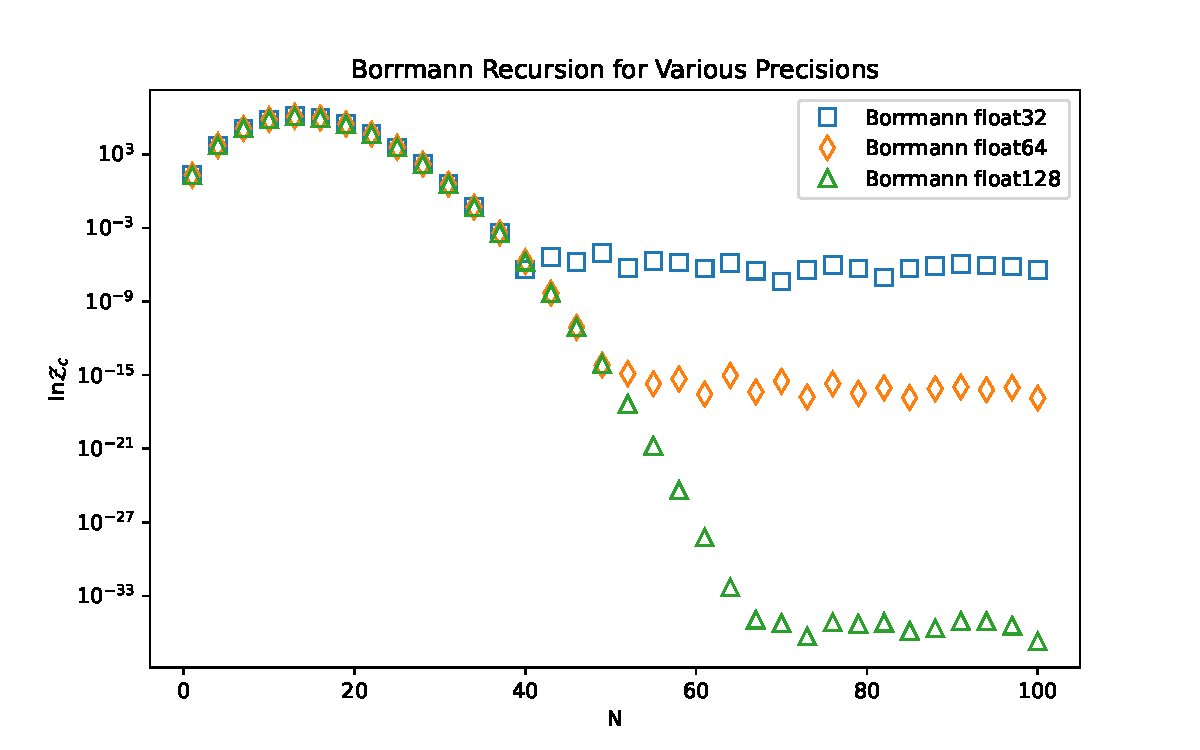
\includegraphics[scale=0.6]{figures/pdf/Borrmann accuracy.pdf}
%     \caption{The solution for the Borrman recursive relation of the canonical partition function for different machine precisions. As $N$ increases, the required precision to accurately find the partition function also increases. The breakdown of the recursion is only delayed by the precision used. Therefore, this is numerically expensive to calculate for $N>60$. Figure adapted from \cite{Jiang}.}
%     \label{fig:BorrmannAcc}
% \end{figure}
As shown, to accurately calculate the partition function, the summation must either be truncated before it fails, or the numerical precision used must be increased. The latter method becomes very computationally expensive from a memory standpoint and takes a long time. 
In addition to this, the $(-1)^{k+1}$ term creates another problem. This term means that the summation is constantly changing signs creating a sort of sign problem. Once again, fixing this problem requires truncation or an increase in numerical precision. Truncating the summation may fail to completely describe the partition function, and higher precision requires more memory. Given these problems, it is necessary to use a different approach. 

Instead of using this general recursive relation, it is helpful to see if there are any specific cases that can be solved. The easiest example would be that of fermions confined in a harmonic trap. An exact solution was found for this spectrum by Sch\"onhammer \cite{Schon1996}. For the one dimensional simple harmonic oscillator, the partition function was found to be
\begin{equation}
    Z_N=e^{-\beta E_N^0} \prod_{m=1}^N \frac{1}{1-e^{-\beta m\Delta}} \label{schoneqn}
\end{equation}
where $\Delta$ is the spacing between equidistant energy levels and $E_N^0$ is the ground state energy \cite{Schon1996}. This is the exact solution for the canonical partition function of a linear spectrum and provides a result that other methods can use to check their accuracy.

While this solution works for the specific cases of a linear energy spectrum, a general solution is still needed for other energy spectra. This has been worked out by Barghathi et al. \cite{Hatem2020}. The canonical partition function can be calculated using a summation.
\begin{equation}
    Z_N=\sum_{k=k_{min}}^{k_{max}} Z_k(S^{(1)})Z_{N-k}(S^{(2)})
    \label{eq:ZNcombine}
\end{equation}
where $S$ denotes a spectrum that is a union of disjoint subspectra \cite{Hatem2020}. This can be written as 
\begin{gather}
    S=S^{(1)}\cup S^{(2)}.
\end{gather}
Using this spectral formulation, the partition function summation can be written more specifically as 
\begin{equation}
    Z_N=\sum_{k=0}^N Z_k(\{\epsilon_1,\epsilon_2,...\epsilon_j\})Z_{N-k}^{\backslash \{\epsilon_1,\epsilon_2,...\epsilon_j\}} \label{newZN}
\end{equation}
where the $\backslash \{\epsilon_1,\epsilon_2,...\epsilon_j\} $ denotes the energy levels excluded from the spectrum of the particular partition function. Now let each spectrum $S^{(j)}$ consist of a single energy level. For non-interacting fermions, the partition function of a system with a single energy level is
\begin{equation}
    Z_k(\{j\})=\begin{cases} e^{-\beta \epsilon_j k} & 0\leq k \leq 1\\0 & \text{otherwise}.\end{cases}
\end{equation}
By substituting this into Eq.\@ (\ref{newZN}) we see that
\begin{equation}
    Z_N=Z_N^{\backslash\{j\}}+e^{-\beta\epsilon_j}Z_{N-1}^{\backslash\{j\}}. \label{hatemrr}
\end{equation}
This equation can be understood by looking at each term on the right side. On the left side of the addition, the $Z_N^{\backslash\{j\}}$ term is the canonical partition function of $N$ particles with no particle in the $j$th energy level. This represents the complementary probability, or the probability that energy level $\epsilon_j$ is unoccupied. The term on the right hand side has a Boltzmann probability for energy level $\epsilon_j$ times the canonical partition function of $N-1$ particles with no particle at the $j$th energy level. The Boltzmann term introduces the probability of occupying state $j$ with a particle, so the total number of particles on the right hand side of the addition is $N$, the same as the left. The state that is excluded from the partition function is reintroduced meaning that this term is the probability that energy level $\epsilon_j$ is occupied. Since the state can only be occupied or unoccupied for fermions, we can recognize that the full partition function is a sum of the unoccupied and occupied terms, or the full probability. 

To understand this better, let's consider another simple example with only two energy levels $\epsilon_1$ and $\epsilon_2$. The canonical partition function is 
\begin{equation}
    Z_N = \begin{cases}
    1 & N=0\\
    e^{\epsilon_1}+e^{\epsilon_2} & N=1\\
    e^{\epsilon_1+\epsilon_2} & N=2
    \end{cases}.
\end{equation}
Now using this formulation from above, break down the full spectrum into two subsectra given as 
\begin{gather}
    Z_N^1=\begin{cases}1&N=0\\e^{\epsilon_1}& N=1\end{cases}\\
    Z_N^2=\begin{cases}1&N=0\\e^{\epsilon_2}& N=1\end{cases}.
\end{gather}
Now the partition function corresponding to each $N$ can be calculated using Eq. \ref{hatemrr}.  
\begin{gather}
    Z_0= (1)(1)=1\\
    Z_1= (1)(e^{-\beta\epsilon_1})+(e^{-\beta\epsilon_2})(1)=e^{-\beta\epsilon_1}+e^{-\beta\epsilon_2}\\
    Z_2=(e^{-\beta\epsilon_1})(e^{-\beta\epsilon_2})=e^{-\beta\epsilon_1-\beta\epsilon_2}.
\end{gather}
Putting these values together yields 
\begin{equation}
    Z_N = \begin{cases}
    1 & N=0\\
    e^{\epsilon_1}+e^{\epsilon_2} & N=1\\
    e^{\epsilon_1+\epsilon_2} & N=2
    \end{cases}.
\end{equation}
which is exactly what was calculated before. So the canonical partition function can indeed be found through this method.